\documentclass{standalone}
\usepackage{chez}

\begin{document}
\chapter{September 04, 2020}
Last time, we computed the homology group of a combinatorial object,
a directed graph. However, there are two problems that arise:
\begin{enumerate}
  \item We want to handle higher dimensional objects.
  \item We want to handle topological spaces and
  not just combinatorial objects.
\end{enumerate}

Let's try to work on the first issue.
\begin{definition}
  A \vocab{semisimplicial set} \(X\) is
    a sequence of sets \(X_0, X_1, X_2, \dots\) and
    functions
    \begin{align*}
      d_0, d_1 &\colon X_1 \to X_0 \\
      d_0, d_1, d_2 &\colon X_2 \to X_1 \\
      &\shortvdotswithin{\colon}
      d_0, d_1, d_2, \dots, d_n &\colon X_n \to X_{n-1} \\
      \MTFlushSpaceAbove
      &\vdotswithin{\colon}
    \end{align*}
  that satisfy the \vocab{simplicial identities}
  \[
    d_i d_j = d_{j - 1} d_i \quad
    \text{whenever \(i < j\)}.
  \]

  These sets \(X_n\) are called the \vocab{\(n\)-simplices}, and the maps
  \(d_i\) are called the \vocab{face maps}.
\end{definition}

\begin{example}
  A semisimplicial set with \(\nullset = X_2 = X_3 = \cdots\), etc.\
  is just a directed graph
  \begin{align*}
    X_0 &= \set{\text{vertices}} \\
    X_1 &= \set{\text{edges}}
  \end{align*}
  with
  \[
    d_0, d_1 \colon X_1 \to X_0,
  \]
  with \(d_0\) mapping an edge to the ``target''
  and \(d_1\) mapping an edge to the ``source''.
\end{example}

\begin{example}
  If we have the following combinatorial structure:
  \begin{center}
    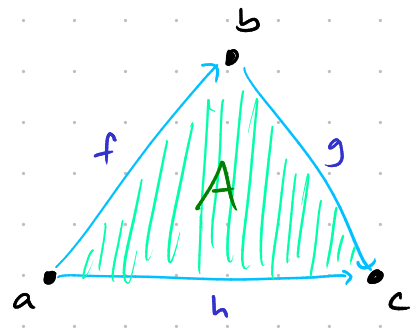
\includegraphics[width=0.3\textwidth]{18_905-200904-2.png} % chktex 8
  \end{center}
  This represents the semisimplicial set with
  \begin{align*}
    X_0 &= \set{a, b, c} \\
    X_1 &= \set{f, g, h} \\
    X_2 &= \set{A} \\
    X_3 = X_4 &= \nullset. \\
    \MTFlushSpaceAbove
    &\vdotswithin{=}
  \end{align*}
  Then we have the functions
  \[
    d_0, d_1 \colon X_1 \to X_0
    \qquad \text{and} \qquad
    d_0, d_1, d_2 \colon X_2 \to X_1
  \]
  where
  \begin{align*}
    d_0 f &= b &
      d_1 f &= a &
      d_0 A &= g \\
    d_0 g &= c &
      d_1 g &= b &
      d_1 A &= h \\
    d_0 h &= c &
      d_1 h &= a &
      d_2 A &= f.
  \end{align*}
  To see why \(d_0, d_1, d_2\) act on \(A\) the way they do,
  note that the simplicial identities require
  \[
    d_0 d_2 A = d_1 d_0 A.
  \]
  The element in \(X_0\) that must equal these two values must be a source
  and a target, so it must be \(b\). The values of \(d_0 A\), \(d_1 A\),
  and \(d_2 A\) follow.
\end{example}

Note that it's important that the edges go forward from \(a \to b \to c\)
and backwards from \(c \gets a\). Otherwise, the simplicial identity would
not be able to uniquely define \(d_0, d_1, d_2\) on \(A\).

\section{Homology}
If \(X\) is a semisimplicial set, then let \(S_n(X)\) be the abelian group
of \vocab{singular \(n\)-chains},
the free abelian group generated by the set \(X_n\) of \(n\)-simplices.

\begin{definition}
  For \(n \geq 1\), the \vocab{boundary operators} are group homomorphisms
  \[
    \partial_n \colon S_n(X) \to S_{n - 1}(X)
  \]
  defined by the generators \(\sigma \in X_n\) where
  \[
    \sigma \mapsto \sum_{k = 0}^{n} (-1)^k d_k \sigma.
  \]

  We also define \(\partial_0 \colon S_0(X) \to 0\) to be
  the zero homomorphism.
\end{definition}

\begin{definition}
  Suppose \(X\) is a semisimplicial set. The group of \vocab{\(n\)-cycles}
  in \(X\), denoted by \(Z_n(X)\) is the kernel of \(\partial_n\).
  
  The group of \vocab{\(n\)-boundaries} in \(X\), denoted \(B_n(X)\),
  is the image of \(\partial_{n+1}\).
\end{definition}

\begin{exercise}[On homework]
  \(B_n(X)\) is a subgroup of \(Z_n(X)\), which is in turn
  a subgroup of \(S_n(X)\).
\end{exercise}

We can therefore define the \vocab{\(n\)th singular homology group} of \(X\),
\[
  H_n(X) = Z_n(X) / B_n(X) = \frac{\ker \partial_n}{\img \partial_{n+1}},
\]
which is an abelian group because the quotient of an abelian group is abelian.
This intuitively measures the number of \(n\)-dimensional holes in \(X\).

% % % % % % % % % % % % % % % % % % % % % % % % % % % % % % % % % % % % % % % %
\section{Topological spaces}
\begin{question}
  How do we get a semisimplicial set out of a topological space?
\end{question}

The basic tool we will use are simplices.
\begin{definition}
  For \(n \geq 0\), the \vocab{standard \(n\)-simplex} \(\Delta^n\) is
  the subspace of \(\RR^{n+1}\) that is the convex hull of the standard basis
  \(\set{e_0, \dots, e_n}\) in \(\RR^{n+1}\). In particular,
  \[
    \Delta^n = \set*{\sum t_i e_i \mid \sum t_i = 1, t_i \geq 0}
      \subseteq \RR^{n+1}.
  \]
  The \(t_i\) are sometimes called \vocab{barycentric coordinates}.
\end{definition}

\begin{example}
  \(\Delta^1 \subseteq \RR^2\) is
  the line segment from \((1, 0)\) to \((0, 2)\).

  \(\Delta^2 \subseteq \RR^3\) is
  the triangle with vertices \(\set{(1, 0, 0), (0, 1, 0), (0, 0, 1)}\).
\end{example}

\begin{definition}
  For a topological space \(X\), a \vocab{singular \(n\)-simplex in \(X\)}
  is a continuous map \(\sigma \colon \Delta^n \to X\).
  We will often drop the adjective ``singular''.
  Let \(\Sing_n(X)\) be the set of all \(n\)-simplices in \(X\).
\end{definition}

We can assemble these into a semisimplicial set.
In particular, there are maps \(d_i \colon \Sing_n(X) \to \Sing_{n-1}(X)\)
that come from ``forgetting'' the basis element \(e_i\).
In particular, we have the function \(d_1 \colon \Delta^2 \to \Delta^1\)
that takes the segment (\(\Delta^1\)) that does not include
the vertex corresponding to \(1\).
So given \(\sigma \colon \Delta^2 \to X \in \Sing_2(X)\),
we can restrict \(\sigma\) to \(d_1 \Delta^2 = \Delta^1\),
giving a map \(\Delta^1 \to X \in \Sing_1(X)\).
\begin{align*}
  d_1 \colon& \Sing_2(X) \to \Sing_1(X) \\
    & \sigma \to \sigma\mathord\vert_{d_1 \Delta^2}
\end{align*}
Therefore, \(\Sing(X)\), the collection of all of the \(\Sing_n\) sets,
is a semisimplicial set.

\begin{remark}
  For more intuition, look at Hatcher's treatment of \(\Delta\)-complexes
  (another name for semisimplicial set).
\end{remark}

\begin{definition}
  If \(X\) is a topological space, we can define
  \begin{align*}
    S_n(X) &= S_n(\Sing X), &
    Z_n(X) &= Z_n(\Sing X), &
    B_n(X) &= B_n(\Sing X), \qquad \text{and} &
    H_n(X) &= H_n(\Sing X).
  \end{align*}
\end{definition}

Overall, we are transforming geometric objects into combinatorial objects,
and then in turn transforming them into algebraic objects so that they are
easier to study.
\[
  \begin{tikzcd}
    \parbox[t]{2.8cm}{\centering Topological spaces (geometric)}
      \arrow[r, "\Sing"] &
    \parbox[t]{3cm}{\centering Semisimplicial sets (combinatorial)}
      \arrow[r, "H_n"] &
    \parbox[t]{2.5cm}{\centering Abelian groups (algebraic)}
  \end{tikzcd}
\]


\end{document}
